\section{Additional Experimental Details}

\subsection{SVGD Algorithm on NumPyro}
\label{ssect:svgd-npy}

SVGD is an algorithm that allows us to generate samples from the posterior distribution and perform inference. As a result, the SVGD algorithm can be used in probabilistic programming languages as another method to perform variational inference. However, the original SVGD algorithm uses the posterior probability directly, which for more general purposes, may not be feasible to compute. It is also inconvenient for the users of the algorithm if the posterior has to be specified directly for each inference problem to be conducted.

To perform variational inference, NumPyro provides a method to track the evidence lower bound (ELBO) of some model parameter, and perform auto-differentiation of the function. While the SVGD algorithm in the paper attempts to minimise the true posterior, in the implementations of SVGD found the ELBO is used as the optimisation objective instead. In theory, the SVGD algorithm will still work, returning points that minimises the ELBO (rather than the true posterior) but are also more spread out. 

Additionally, using the entire dataset to compute the ELBO in each timestep is too costly. As a result, in each update step, the algorithm will subsample some number of training data, and use the subset of data to compute the approximate ELBO. This is equivalent to the use of batches in stochastic gradient descent.

We note that NumPyro is closely related to Pyro. However, the main difference is NumPyro uses JAX and NumPy in the backend, while Pyro uses PyTorch. Since we are not running experiments on GPUs, we chose to run the experiments on NumPyro which is more lightweight.

We also note that there seem to be fewer examples of usages of SVGD in practice, as seen in the NumPyro documentation pages where the tutorials favor sampling algorithms such as NUTS or simple variational inference algorithms more. This may be down to the fact that for practitioners, the SVGD algorithm can be seen as more complex and harder to tune than other simpler inference algorithms, while also not providing a large increase in performance. For example, in our tests on small-scale logistic regression algorithms, MCMC-based algorithms perform just as well as SVGD, therefore there was little reason to use it over simpler MCMC algorithms. 

\subsection{SVGD and SGLD on Covertype}
Both algorithms sometimes experience computational instability when computing the gradient of the log-likelihood of the posterior, even using the official implementation of SVGD. However, SVGD encounters much fewer errors during the same amount of trials than SGLD. Interestingly, when the scaling factor in SGLD is tuned down, the algorithm becomes much more stable. Specifically, the scaling factor for the gradient of the log-likelihood in SGLD is $\frac{N}{n}$, where $N$ is the total amount of data and $n$ is batch size. Due to the small batch size (replicating the batch size in the original paper) and large dataset size, it has been noticed that this choice of scaling factor is often the cause of overflows in the debugger. To ensure computational stability, the scaling factor is clipped to less than $10^2$.

\subsection{Bayesian Logistic Regression Tests}\label{ssect:bylog-data}

We present the results from the small-scale logistic regression tasks using the NUTS algorithm and also both implementations of the SVGD algorithm. In Table \ref{tab:logist-acc}, we can see that all three algorithms perform about as well as each other on these tests. However, the SVGD algorithm on NumPyro requires a much higher running time, as seen in Table \ref{tab:logist-time}. 

\begin{table}[t]
    \centering
    \resizebox{\textwidth}{!}{
    \begin{tabular}{|c|ccc|ccc|}
\hline
 & \multicolumn{3}{|c|}{Accuracy} & \multicolumn{3}{|c|}{Average log-likelihood} \\
\hline
Dataset & NUTS & SVGD (NumPyro) & SVGD (Original) & NUTS & SVGD (NumPyro) & SVGD (Original)\\
\hline
banana & 0.555 \pm 0.019 & 0.528 \pm 0.020 & 0.556 \pm 0.032 & -0.686 \pm 0.004 & -0.689 \pm 0.005 & -0.689 \pm 0.001 \\
image & 0.834 \pm 0.004 & 0.830 \pm 0.003 & 0.825 \pm 0.004 & -0.425 \pm 0.005 & -0.426 \pm 0.006 & -0.418 \pm 0.007 \\
ringnorm & 0.759 \pm 0.008 & 0.762 \pm 0.007 & 0.762 \pm 0.003 & -0.514 \pm 0.008 & -0.514 \pm 0.008 & -0.517 \pm 0.004 \\
splice & 0.843 \pm 0.007 & 0.823 \pm 0.006 & 0.832 \pm 0.005 & -0.351 \pm 0.011 & -0.476 \pm 0.025 & -0.392 \pm 0.013 \\
titanic & 0.791 \pm 0.006 & 0.791 \pm 0.006 & 0.785 \pm 0.011 & -0.505 \pm 0.009 & -0.505 \pm 0.010 & -0.570 \pm 0.013 \\
twonorm & 0.973 \pm 0.001 & 0.973 \pm 0.001 & 0.973 \pm 0.002 & -0.070 \pm 0.003 & -0.070 \pm 0.003 & -0.089 \pm 0.010 \\
waveform & 0.881 \pm 0.010 & 0.874 \pm 0.010 & 0.779 \pm 0.012 & -0.265 \pm 0.015 & -0.266 \pm 0.014 & -0.450 \pm 0.017 \\
\hline
\end{tabular}
}
    \caption{Accuracy and log-likelihood obtained from each algorithms on small Bayesian regression tasks.}
    \label{tab:logist-acc}
\end{table}


\begin{table}[t]
    \centering
    \begin{tabular}{|c|ccc|}
\hline
 & \multicolumn{3}{|c|}{Time (seconds)} \\
\hline
Dataset & NUTS & SVGD (NumPyro) & SVGD (Original) \\
\hline
banana & $2.291 \pm 0.047$ & $18.119 \pm 0.819$ & $0.731 \pm 0.011$ \\
image & $3.438 \pm 0.141$ & $19.594 \pm 0.408$ & $1.136 \pm 0.005$ \\
ringnorm & $2.974 \pm 0.054$ & $23.376 \pm 0.436$ & $1.190 \pm 0.004$ \\
splice & $12.227 \pm 0.649$ & $29.474 \pm 0.515$ & $2.301 \pm 0.007$ \\
titanic & $2.005 \pm 0.029$ & $16.930 \pm 0.382$ & $0.756 \pm 0.017$ \\
twonorm & $2.962 \pm 0.036$ & $22.985 \pm 0.067$ & $1.181 \pm 0.003$ \\
waveform & $4.732 \pm 0.117$ & $22.282 \pm 0.392$ & $1.230 \pm 0.006$ \\
\hline
\end{tabular}
    \caption{Average time required to run each algorithms on small Bayesian regression tasks.}
    \label{tab:logist-time}
\end{table}

\subsection{Bayesian Neural Network Tests}\label{ssect:bnn-time}

In Table \ref{tab:bnn_time}, we report the average time to run each of the dataset training with each algorithm. We can see that amongst the three algorithms, the original implementation of SVGD runs the fastest. This is due to the fact that the posterior distribution is computed in closed form for the algorithm, unlike the SVGD algorithm with ELBO objective, which requires more time for ELBO estimation.

\begin{table}[h]
\centering
\begin{tabular}{|c|ccc|}
\hline
 Dataset & PBP & SVGD (original) & SVGD (NumPyro)  \\
 \hline
Boston & $25.926 \pm 0.273$ & $8.193 \pm 0.485$ & $38.177 \pm 0.537$ \\
Concrete & $47.896 \pm 0.502$ & $13.718 \pm 0.298$ & $66.020 \pm 0.974$ \\
Energy & $34.394 \pm 0.205$ & $9.857 \pm 0.330$ & $49.220 \pm 0.564$ \\
Kin8nm & $36.341 \pm 0.781$ & $10.881 \pm 0.393$ & $17.719 \pm 0.634$ \\
Naval & $52.571 \pm 0.142$ & $19.052 \pm 0.157$ & $26.480 \pm 0.299$ \\
Power & $39.195 \pm 0.217$ & $12.299 \pm 0.394$ & $18.067 \pm 0.541$ \\
Protein & $209.791 \pm 1.405$ & $89.086 \pm 0.612$ & $147.737 \pm 3.409$ \\
Wine & $29.518 \pm 0.078$ & $9.160 \pm 0.034$ & $16.557 \pm 0.170$ \\
Yacht & $6.907 \pm 0.064$ & $1.757 \pm 0.076$ & $7.763 \pm 0.174$ \\
\hline
\end{tabular}
\caption{Average time per run (in seconds) on test data for each algorithms on BNN tasks.} 
\label{tab:bnn_time}
\end{table}

\label{ssect:bnn-epoch}

We also show how training is affected as the algorithm runs more epochs. In Figure \ref{fig:bnn-epoch}, we show the results when an instance of the BNN training is trained for up to a certain number of epochs. We can see that given the training is conducted for long enough, the SVGD algorithm will eventually ``catch up" to the PBP algorithm in terms of performance.

\begin{figure}[H]
    \centering
    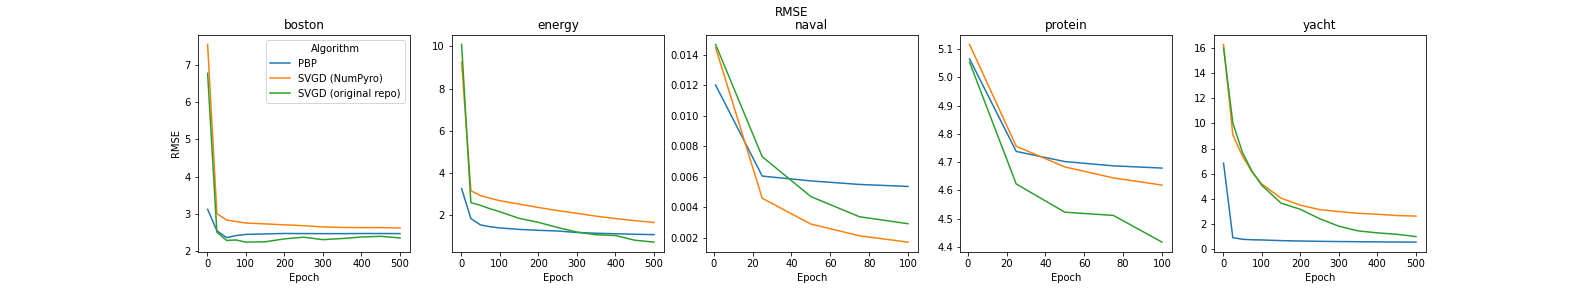
\includegraphics[width=\textwidth]{figs/bayesian_epoch_RMSE.png}
    \newline
    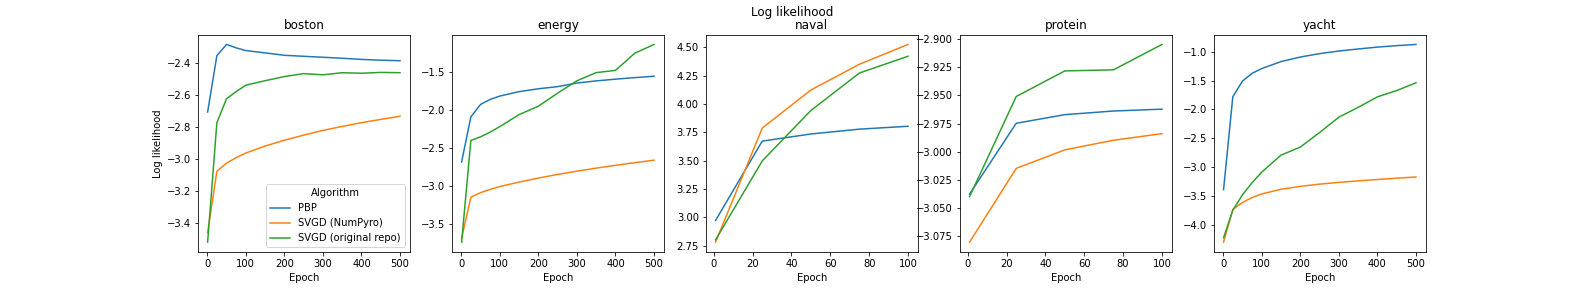
\includegraphics[width=\textwidth]{figs/bayesian_epoch_Loglikelihood.png}
    \caption{The trend in accuracy and log likelihood value for the inferred weights as the number of epochs changes, for some instances of the dataset.}
    \label{fig:bnn-epoch}
\end{figure}